\section{DATA PREDICTIVE CONTROL}
\label{S:dpc}

\textcolor[rgb]{0,0,1}{The central idea behind DPC is to obtain control-oriented models using machine learning methodologies, and formulate the control problem in a way that Receding Horizon Control (RHC) can still be applied and the optimization problem can be solved efficiently. In this paper Regression Trees and Random Forests are considered (see Appendix ??? for details).}

\textcolor[rgb]{0,0,1}{To this aim, let an historical dataset $(\X,\Y)$, created using building measurements, be given to be used in the Regression Trees and Random Forests training process.
Let $|(\X,\Y)| = n$, be the number of samples in the dataset.
$\X = \{(x(k),u(k),d(k))\}$, $\forall k = 1,\ldots,n$, is the set of samples $(x(k),u(k),d(k))$, measured at each time instant $k$, where $x(k)\in\mathbb{R}^{n_x}$ is the vector of the state variables, $u(k)\in\mathbb{R}^{n_u}$ is the vector of the input variables and $d(k)\in\mathbb{R}^{n_d}$ is the vector of the disturbance variables.
$\Y = \{y(k)\},\ \forall k = 1,\ldots,n$, is the set of samples $y(k)$, measured at each time instant $k$, where $y(k)\in\mathbb{R}^{n_y}$ is the vector of the output variables.
We consider $\X$ as the set of predictor variables (or features) and $\Y$ as the set of response variables.
As an example, the response variables can be represented by the power consumption or the room temperatures evolution, while the predictors can be represented by the weather forecast, as the disturbance, the set-points information and building schedules, as the inputs, and room temperatures, as the states. 
Our goal is to learn a data-driven models, using Regression Trees and Random Forests, that relate the value of the response variables with the value of the predictor variables, and that can be used to set up an MPC problem.
}

\textcolor[rgb]{0,0,1}{To do this, we want to derive a model with a closed-form expression of the following form:
\begin{equation}\label{E:GenericModel}
	y(k)=f(x(k),u(k),d(k)),
\end{equation}
where $f$ is an analytical expression that describes the system's dynamics.
\textbf{We want to remark that $y$ can be considered as both a state variable evolution, i.e. $y(k) = x(k+1)$, and a variable that is function of $x$, $u$ and $d$ but is not one of them, as for example is the case of the power. We consider this aspect in Sections \ref{S:proof}, \ref{S:casestudy} and \ref{S:realCaseStudy}. IMPROVE!!!!!!!!!!!!!!!}.
The issue that arises, when using Regression Trees and Random Forests, is that $f$ does not have a closed-form expression, hence \eqref{E:GenericModel} is not suitable for control and optimization.
One possibility could be to look for sub-optimal solutions using evolutionary algorithms \cite{Kusiak2009}, i.e. using heuristics.
In this section we provide a new methodology to determine a closed-form expression for $f$ by manipulating the dataset, as shown starting from Section \ref{SS:sepvar}.}


\subsection{Dataset splitting}
\label{SS:sepvar}

\textcolor[rgb]{0,0,1}{The dataset splitting consists of partitioning the features set $\X$ into the sets $\X^c = \{u(k)\}\subset\X,\ \forall k=1,\ldots,n$, containing the control (or manipulated) variables, and $\X^d = \{(x(k),d(k))\}\subset\X,\ \forall k=1,\ldots,n$, containing the disturbance and state (or non-manipulated) variables.
The union of the two sets forms the full feature set oftraining, i.e. $\X \equiv \X^c \cup \X^d$.
%Our goal is to replace a model-based controller with a data-driven controller, where the latter depends only on the historical sensor data. 
%These measurements could directly represent one or more states in the model-based control framework. We denote these as outputs $\Y \in \R$ for training, i.e. a $\Y$ represents a particular output and we can have separate models for multiple outputs. We define the number of training samples by $|(\X,\Y)| = n$.
Using this splitting methodology, the training process is divided into two steps:
	\begin{enumerate}
		\item the trees and the forests are trained only using $\X^d$, which also eases the computational complexity.
			  It is important to note that besides external disturbance and the state measurements, $\X^d$ can also contains autoregressive terms of the output variables in $\Y$;
		\item in each leaf of the tree (or in each leaf of each the tree of the forest), a linear regression model is trained as a function of the inputs variables in $\X^c$.
		As we shall see in Section~\ref{SS:dpcrt} and \ref{SS:dpcrf}, the second step reduces the run-time control problem into a convex program.
	\end{enumerate}
This process is illustrated in Figure~\ref{F:dpc-sepvars} (left). For the sake of simplicity only trees are considered, but the same holds for the forests. The meaning of the variable $j$ in the linear model in the figure will be clear in the next section.
In Figure~\ref{F:dpc-sepvars} (right), the step 1 of the training process uses also the input variables, i.e. the classical training process without the dataset splitting.
The reason why this latter approach is not suitable for control will be discussed at the end of Section \ref{SS:dpcrt}.
}

\subsection{DPC-RT: DPC with Regression Trees}
\label{SS:dpcrt}
When the data has lots of features, which interact in complicated, nonlinear ways, assembling a single global model such as linear or polynomial regression can be difficult, and can lead to poor response predictions.
\textcolor[rgb]{0,0,1}{As discussed before, an approach to non-linear regression is to partition the data space into smaller regions, where the interactions are more manageable. }
This partition is repeated recursively until we finally get to small chunks of the data space where we can fit simple (eg. linear parametric) models. 
%Therefore, in \eqref{E:sepvars}, the global model $f$ has two parts: the recursive partition $g$, and a linear (and convex) model $h$ for each cell of the partition.

\begin{figure}[t!]
	\centering
	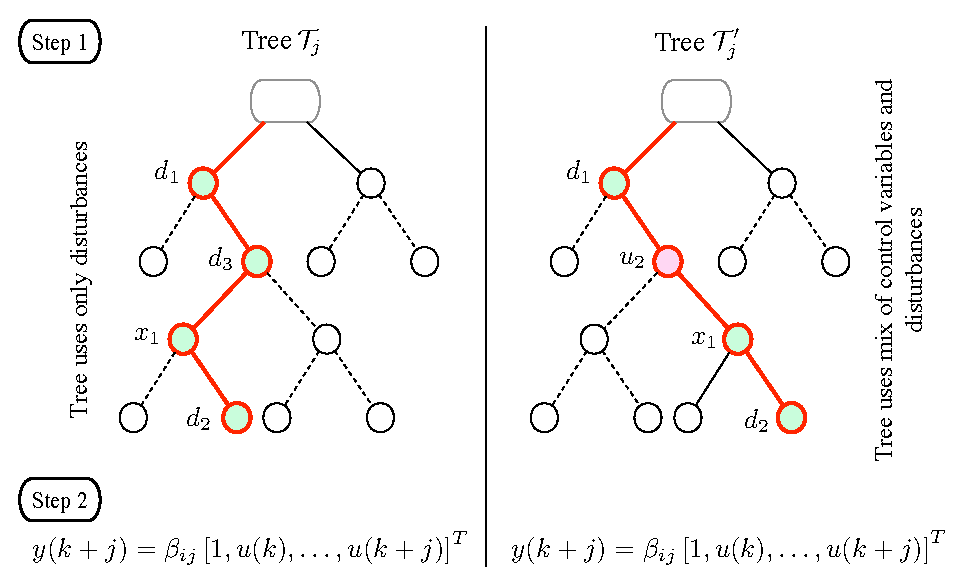
\includegraphics[width=20pc]{figures/dpc-sepvars.eps}
	\caption{Dataset splitting. \textit{Step 1:} Tree $\mathcal{T}_1$ is trained only with variables in $\X^d$ as the features. Tree $\mathcal{T}_2$ uses both the disturbances and states in $\X^d$, and the control variables in $\X_c$ for splitting. It is thus not computationally suitable for control. \textit{Step 2:} In the leaf $\ell_i$ of the trees, a linear regression model parametrized by $\beta_i$ is defined as a function only of the control variables.}
	\captionsetup{justification=centering}
	\label{F:dpc-sepvars}
\end{figure}

\textcolor[rgb]{0,0,1}{Now, in order to have a model that can be used for prediction over an arbitrary long horizon in an MPC problem, our goal is to predict, at time $k$, the output $y$ for next $N$ time steps, i.e. $y(k),\ldots,y(k+N)$, where $N$ is the control horizon, given the state measurements, i.e. $x(k)$, and the disturbance forecast, i.e. $\tilde d(k),\ldots,\tilde d(k+N)$, at time $k$.
For the sake of simplicity and without any loss of generality, in the following, we consider only a single output, i.e. $y(k)\in\mathbb{R}$ (or $n_y = 1$).
However, as we will see in Sections \ref{S:casestudy} and \ref{S:realCaseStudy}, multiple trees (or forests) can be built for multiple outputs.
Applying the dataset splitting, we build $N$ regression trees using CART procedure \cite{Breiman1984} (see also Appendix for more details), such that the output $y(k+j)$ of the $j^{th}$ tree depends upon the previous $\delta_d$ disturbances, and on the state at instant $k$ and its $\delta_x$ regressive terms:
\begin{equation}\label{E:model_tree}
\T_j = \mathit{f}_{\mathrm{tree}} \left( d(k+j-\delta_d),\ldots,d(k+j),x(k-\delta_x),\ldots,x(k)  \right),\ j=1,\ldots,N,
\end{equation}
with $\left( d(k+j-\delta_d),\ldots,d(k+j),x(k-\delta_x),\ldots,x(k)  \right)\in\X^d,\ k=1,\ldots,n$, and $\mathit{f}_{\mathrm{tree}}$ representing the tree structure.
Then, the linear models, as functions of the inputs variables $u\in\X^c$, in each leaf of the trees $\T_j,\ j=1,\ldots,N$, are defined as
\begin{equation}\label{E:model_leaf}
y(k+j) =  \beta_j [1,u(k),\ldots,u(k+j) ]^T,\ j=1,\ldots,N.
\end{equation}}
Note that the coefficients $\beta_j$ are different for each leaf.
Equation~\eqref{E:model_leaf} implies that the prediction of output $y(k+j)$ at time $k$ is an affine combination of control inputs from time $k$ to $k+j$.
Thus, we have managed to linearize the original model dynamics via black-box modeling.
\textcolor[rgb]{0,0,1}{One of the advantages of this approach is that this two-step training is done off-line, so the time required to create the models does not affect the control execution in run-time.}

\textcolor[rgb]{0,0,1}{The problem now is: \emph{how to use this modeling framework to set up an MPC problem?} In run-time, given the disturbance forecast and the state measurements at time $k$, i.e. $\tilde d(k+j-\delta_d),\ldots,\tilde d(k+j),x(k-\delta_x),\ldots,x(k)$ given $k$, we can narrow down to a leaf of each tree in \eqref{E:model_tree} to retrieve the linear models in \eqref{E:model_leaf} for each step $j=1,\ldots,N$ of the horizon (see first part of the pseudo code given in Algorithm \ref{A:dpcrt}), as depicted in Figure \ref{F:dpc-sepvars} (left). These models are used to setup the MPC Problem \ref{P:dpcrt}.
In particular, }when a new control action has to be determined, each tree (prediction step) contributes to a linear constraint in the optimization as a replacement for the state dynamics in the case of MPC. Thus, the MPC optimization problem, considering a quadratic cost ($Q \succeq 0, R \succeq 0$) function and the general case of multiple outputs, i.e. $y(k)\in\mathbb{R}^{n_y},\ n_y\geq 1$, can be formulated as:
%\begin{problem}\label{P:dpcrt}
%	\begin{equation}
%		\begin{aligned}
%		\text{min } & \sum_{j=1}^{N} ({\Y}_{\mathrm{k+j|k}})^2 \mathcal{Q} + {\X^c}^T_{\mathrm{k+j-1|k}} \mathcal{R} {\X^c}_{\mathrm{k+j-1|k}} + \lambda\epsilon_j\\
%		\text{s.~t. } & \ \ \ \ \ \Y_{\mathrm{k+j|k}} =  \beta^T [1,\X^c_{\mathrm{k|k}},\dots,\X^c_{\mathrm{k+j-1|k}} ]^T \\
%		& \ \ \ \ \ \ \ \ \ \ \ \ \ \ \ \underline{\X}^c \leq \X^c_{\mathrm{k+j-1|k}} \leq \bar{\X}^c\\ 
%		& \ \ \ \ \ \ \ \ \ \ \ \ \underline{\Y}-\epsilon_j \leq \Y_{\mathrm{k+j|k}} \leq \bar{\Y} + \epsilon_j\\\
%		& \ \ \ \ \ \ \ \ \ \ \ \ \ \ \epsilon_j \geq 0, \ j = 1,\dots,N.
%		\end{aligned}
%		\label{E:dpcrt}
%	\end{equation}
%\end{problem}
\begin{problem}\label{P:dpcrt}
	\begin{equation}
	\begin{aligned}
	& \underset{u_{k+j}}{\text{minimize}} & & \sum_{j=1}^{N} y^\top_{k+j} Q y_{k+j} + u^\top_{k+j} R u_{k+j} + \lambda\epsilon_j \\
	& \text{subject to }                  & & y_{k+j}     =   \beta_j [1,u_{k},\ldots,u_{k+j} ]^\top                             \\
	&                                     & & u_{k+j}    \in  \mathcal{U}                                                        \\
	&                                     & & |y_{k+j}|  \leq \bar{y}_{k+j} + \epsilon_j 										 \\
	&                                     & & \epsilon_j \geq  0							                                     \\
	&                                     & & j           =    1,\ldots,N.            									         \\
	\end{aligned}
	\label{E:dpcrt}
	\end{equation}
\end{problem}

\textcolor[rgb]{0,0,1}{Here, $Q \in \mathbb{R}^{n_y\times n_y}$ and $R \in \mathbb{R}^{n_u\times n_u}$ are weight matrices used to give more importance in the minimization to either $y$ or $u$.
This problem is solved as in the classical MPC formulation, i.e. at each time step $k=1,2,\ldots$ the optimal control sequence $u^*_k,\ldots,u^*_{k+N}$ is computed, and only the first input of the sequence is applied as control input to the system: $u(k) = u^*_k$.
The slack variables $\epsilon_j$ are added to ensure recursive feasibility (since the equality constraint on $y$ is relaxed), i.e. to guarantee that Problem \ref{P:dpcrt} can provide a solution at each step $k=1,2,\ldots$.
$\lambda$ is a weight used to give more importance to bounds violation with respect to $y$, than to the cost function optimization, and viceversa. 
Of course, a different cost function can be chosen depending upon the application, i.e. it can be linear, nonlinear, etc., obviously changing the complexity of the problem.
In the current formulation, the data-driven control problem is reduced to a convex program which is very easy and efficient to solve.}
The pseudo code for DPC-RT is given in Algorithm~\ref{A:dpcrt}.
\textcolor[rgb]{0,0,1}{DPC algorithm is also graphically shown in Figure \ref{F:dpc-algo-rf} for the random forest case, but the same holds for single regression trees.}

\textcolor[rgb]{0,0,1}{\begin{remark}
	 If we did not consider the splitting procedure	of the dataset, and we also used input variables to learn the trees, as in the right side of Figure 1, the resulting
	 model would not have been suitable for control. This is because, since u is the variable we want to optimize, we do not know its value a priori to go through the trees and determine the correct leaves to find the models to use in the RHC problem.
\end{remark}}

\begin{algorithm}[t!]
	\caption{Data Predictive Control with Regression Trees}
	\label{A:dpcrt}
	\begin{algorithmic}[1]
		\State \textsc{Design Time (Off-Line)}
		\Procedure{Model Training using Dataset Splitting}{}
		\State Set $\X^c$ $\gets$ manipulated features
		\State Set $\X^d$ $\gets$ non-manipulated features
		\State Build $N$ predictive trees with $(\X^d,\Y)$ as defined in \eqref{E:model_tree}
		\ForAll{trees $\mathcal{T}_j$}
		\ForAll{the leaves $\ell_i$ of $\mathcal{T}_j$}
		\State Fit $ y(k+j) =  \beta_j \left[1,u(k),\ldots,u(k+j) \right]^T$ as in \eqref{E:model_leaf}
		\EndFor
		\EndFor
		\EndProcedure
		\State \textsc{Run Time}
		\Procedure{Predictive Control}{}
		\While{$k< k_{\mathrm{stop}}$}
		\ForAll{trees $\mathcal{T}_j$}
		\State Determine the leaf $\ell_i$ using $\X^d$ as in \eqref{E:model_tree}
		\State Obtain the linear model at $\ell_i$ trained in \eqref{E:model_leaf}
		\EndFor
		\State Solve optimization problem \ref{P:dpcrt} to determine optimal
		\State control actions $u^*_k,\ldots,u^*_{k+j}$
		\State Apply the first input $u(k)=u^*_k$
		\EndWhile
		\EndProcedure
	\end{algorithmic}
\end{algorithm}

\subsection{DPC-En: DPC with Ensemble Methods}
\label{SS:dpcrf}
Regression trees obtain good predictive accuracy in many domains. However, the models used in their leaves have some limitations regarding the kind of functions they are able to approximate.
The problem with trees is their high variance and that they can overfit the data easily.
A small change $\delta$ in the data can result in a different series of splits and thus violate the acceptable accuracy.
This is the price to be paid for estimating a tree-based structure from the data.


We use ensemble methods \cite{Friedman2001}, in particular Random Forests, to combine the predictions of several independent regression trees in order to improve generalizability and robustness over a single estimator. 
The essential idea is to average many noisy trees to reduce the overall variance in prediction.
We inject randomness into the tree construction in two ways. First, we randomize the features used to define splitting in each tree.
Second, we build each tree using a bootstrapped or sub-sampled data set.
In this way, each tree in the forest is trained on different data, which introduces differences between the trees.
\textcolor[rgb]{0,0,1}{More explicitly, training features $\bar{\X}^d_i\subset\X^d$, $i=1,2,...$ and the in-bag samples (in-bag samples correspond to the data samples which each tree was trained on) are different for each tree in the forest, i.e $|(\bar \X^d_i,\bar\Y_i)|<n$, with $\bar\Y_i\subset\Y$.}

\textcolor[rgb]{0,0,1}{The goal with DPC-En is to replace each tree in Algorithm~\ref{A:dpcrt} by a forest.
This can be done replacing Equations \eqref{E:model_tree} and \eqref{E:model_leaf} with the Equations \eqref{E:model_forest} and \eqref{E:model_leaf_forest} provided in the following:
\begin{equation}\label{E:model_forest}
\F_j = \mathit{f}_{\mathrm{forest}} \left( d(k+j-\delta_d),\ldots,d(k+j),x(k-\delta_x),\ldots,x(k)  \right),\ j=1,\ldots,N,
\end{equation}
with $\left( d(k+j-\delta_d),\ldots,d(k+j),x(k-\delta_x),\ldots,x(k)  \right)\in\X^d,\ k=1,\ldots,n$, and $\mathit{f}_{\mathrm{forest}}$ representing the forest structure.
In particular, as mentioned above, each tree $\T_i$ of each forest $\F_j$ is trained using $(\bar \X^d_i,\bar\Y_i)$.
Then the linear models, as functions of the inputs variables $u\in\bar\X^c_i\subset\X_c$, in each leaf of each tree of the forests $\F_j,\ j=1,\ldots,N$, are defined as
\begin{equation}\label{E:model_leaf_forest}
y(k+j) =  \Theta_{ij} [1,u(k),\ldots,u(k+j) ]^T,\ j=1,\ldots,N.
\end{equation}
Here $(\bar\X^c_i,\bar\Y_i)$ correspond to the in-bag samples for the trees.}

While the off-line training burden in DPC-En is slightly increased compared to DPC-RT, in the control step we exploit the better accuracy, and lower variance properties of the random forests. 
If a forest has $t$ number of trees, given the forecast of disturbances, we have $t$ sets of linear coefficients. We simply average out all the coefficients from all the trees to get one linear model represented by $\hat{\Theta}_j$ for each forest. Note that the averaging step can only be done in run-time, because the leaf of each tree can be narrowed down only when the $\X^d$ is known. Thus, for $N$ forests, we again have exactly $N$ linear equality constraints as in the optimization problem below:

\begin{problem}\label{P:dpcrf}
	\begin{equation}
	\begin{aligned}
	& \underset{u_{k+j}}{\text{minimize}} & & \sum_{j=1}^{N} y^\top_{k+j} Q y_{k+j} + u^\top_{k+j} R u_{k+j} + \lambda\epsilon_j \\
	& \text{subject to }                  & & y_{k+j}      =  \hat{\Theta}_j [1,u_{k},\ldots,u_{k+j} ]^\top                      \\
	&                                     & & u_{k+j}    \in  \mathcal{U}                                                        \\
	&                                     & & |y_{k+j}|  \leq \bar{y}_{k+j} + \epsilon_j 										 \\
	&                                     & & \epsilon_j \geq  0							                                     \\
	&                                     & & j           =    1,\ldots,N.            									         \\
	\end{aligned}
	\label{E:dpcrf}
	\end{equation}
\end{problem}
DPC-En is graphically described in Figure~\ref{F:dpc-algo-rf}.

The ensemble data predictive control (DPC-En) is the first such method to bridge the gap between ensemble predictive models (such as random forests) and receding horizon control. In the next section, we compare DPC-RT and DPC-En to MPC for a building model.

\begin{figure}[t!]
	\centering
	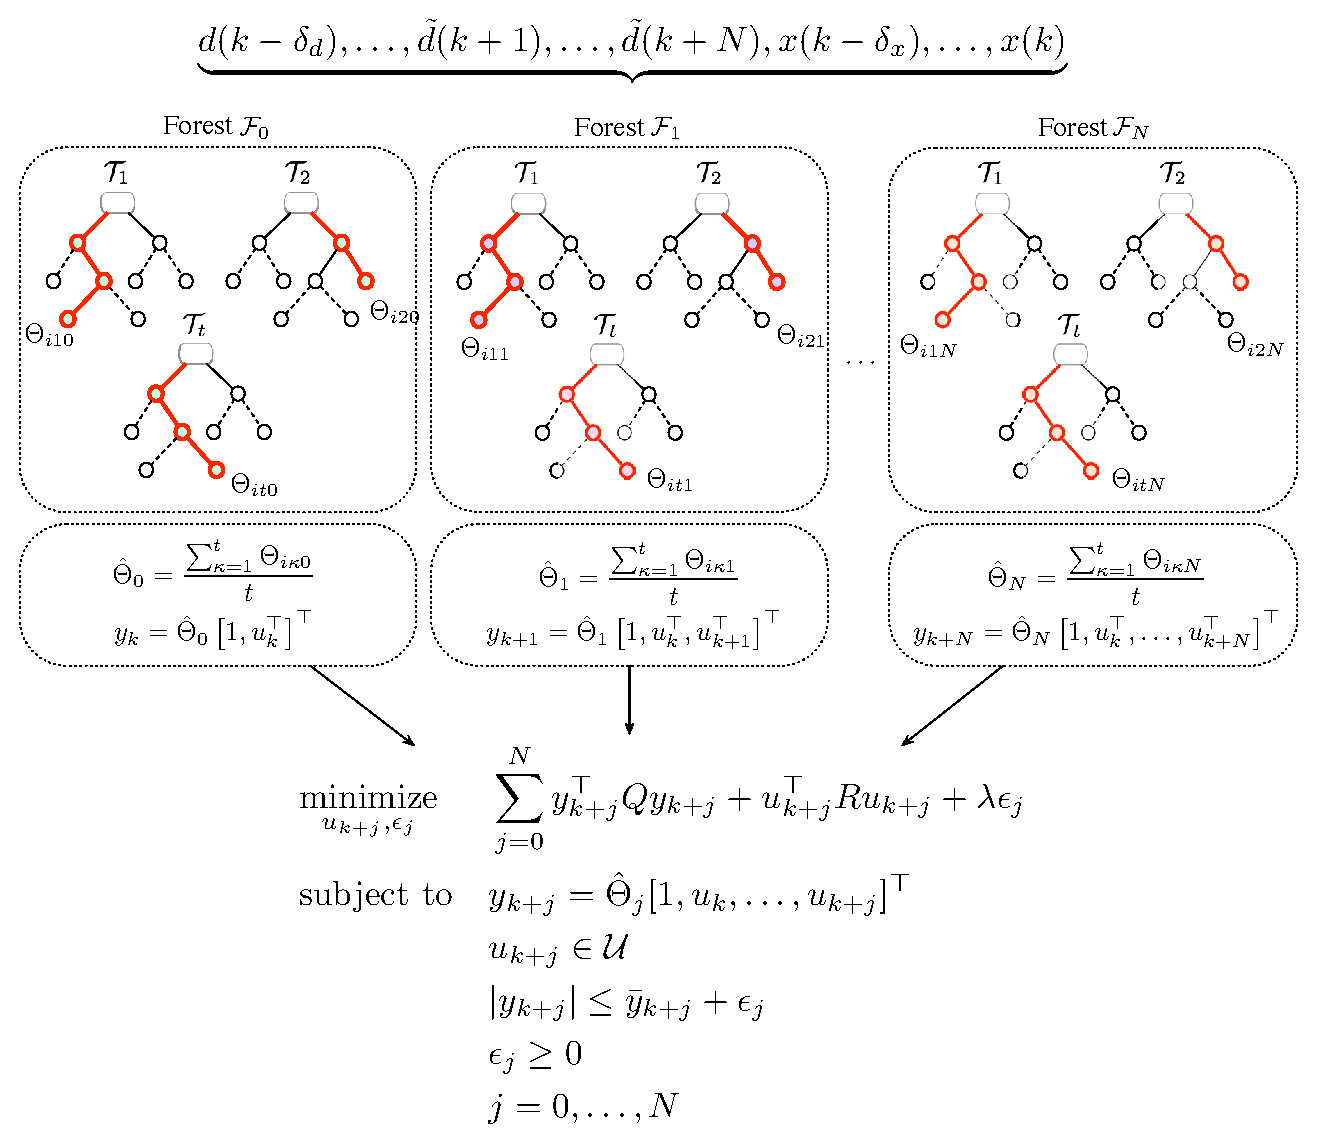
\includegraphics[width=26pc]{figures/dpc-algo-rf.eps}
	\caption{\textcolor[rgb]{0,0,1}{DPC-En: At time $k$, the algorithm uses the forecast of disturbances and the state measurements in $\X^d$ at time $k$ to select linear models $\Theta_1$ to $\Theta_t$ in the leaves of each forest. The linear models in each forest are averaged to calculate a single model represented by $\hat{\Theta}_j$, and act as constraints in the optimization problem. The optimal sequence $u^*_k,\ldots,u^*_{k+N}$, of which only the first element is applied, i.e. $u(k)=u^*_k$, and variables in $\X^d$ at time $k+1$ are calculated to proceed to next step at $k+1$.}}
	\label{F:dpc-algo-rf}
\end{figure}